\documentclass[12pt, authoryear]{elsarticle}
\makeatletter
\def\ps@pprintTitle{%
	\let\@oddhead\@empty
	\let\@evenhead\@empty
	\def\@oddfoot{}%
	\let\@evenfoot\@oddfoot}
\makeatother
%\usepackage{lmodern}
% My spacing
\usepackage{setspace}
\setstretch{1.5}
\usepackage{multirow}
%\DeclareMathSizes{12}{14}{10}{10}
\usepackage[margin=2.5cm]{geometry}    % How to set margins - optimized for 2.5cm      
\usepackage[capposition=top]{floatrow}

% See geometry.pdf to learn the layout options. There are lots.
\geometry{a4paper}                   			% ... or a4paper or a5paper or ... 
\usepackage{enumitem}
\usepackage{mathtools}
%\geometry{landscape}                		% Activate for rotated page geometry
\usepackage[parfill]{parskip}    			% Activate to begin paragraphs with an empty line rather than an indent
\usepackage{graphicx}						% Use pdf, png, jpg, or eps§ with pdflatex; use eps in DVI mode
% TeX will automatically convert eps --> pdf in pdflatex	
\usepackage{flafter}			
\usepackage{setspace}
%\linespread{1.5}
\usepackage[font={}]{caption}
\usepackage[bottom]{footmisc}
\usepackage[capposition=top]{floatrow}   %figure notes
\usepackage{lscape}
%math packages 
\usepackage{amssymb}
\usepackage{fancyhdr}
\usepackage{graphicx,epsf,subfigure}
\usepackage{pstricks,pst-node,psfrag}
\usepackage{amsthm,amssymb,amsmath}
\usepackage{amsmath,bm}

%mathnotes
\newcommand{\bbeta}{\mbox{\boldmath $\beta$}}
\newcommand{\beps}{\mbox{\boldmath $\epsilon$}}
\newcommand{\bX}{\mbox{\boldmath $X$}}
\newcommand{\bY}{\mbox{\boldmath $Y$}}
\newcommand{\bI}{\mbox{\boldmath $I$}}
\newcommand{\N}{\mathcal{N}}
\newcommand{\x}{\textsc{\textbf{x}}}
\newcommand{\xx}{\textsc{x}}
\definecolor{aurometalsaurus}{rgb}{0.43, 0.5, 0.5}
%add figure 
\DeclareGraphicsRule{.tif}{png}{.png}{`convert #1 `dirname #1`/`basename #1 .tif`.png}
\usepackage{rotating}
\usepackage{pdflscape}
\usepackage{hyperref}
\usepackage[round]{natbib}
\definecolor{ashgrey}{rgb}{0.7, 0.75, 0.71}
\usepackage{soul}
\usepackage{animate}

\def\bibsection{\section{References}} %%% Make "References" appear before bibliography
\usepackage{longtable}
\usepackage{hyperref}
\usepackage{tablefootnote}
\usepackage{lscape} 
\usepackage{animate}

\renewcommand{\contentsname}{Table of Contents} % change name from Contents to Table of Contents

\usepackage{titlesec}

\setcounter{secnumdepth}{4}

%_______________________________________________________________________________________________________%
%_______________________________________________________________________________________________________%
%\usepackage[table]{xcolor}% http://ctan.org/pkg/xcolor
%\usepackage{graphicx,multirow}
\usepackage{xcolor,colortbl}
\usepackage{xcolor}
%\usepackage{graphicx,multirow}
\usepackage[capposition=top]{floatrow}
\setcounter{secnumdepth}{4}
\usepackage{tikz}
\begin{document}
	
	\begin{frontmatter}  %
		
		\title{REINFORCEMENT LEARNING FOR AUTOMATED TRADING
		}
		
		\author[Add1]{Reid Falconer}
		\ead{reid.falconer@barcelonagse.eu}
		
		\author[Add1]{Sam MacIntyre}
		\ead{sam.macintyre@barcelonagse.eu}
		
		\author[Add1]{Hector Cano}
		\ead{hector.cano@barcelonagse.eu}

		\author[Add1]{Maximilian Zebhauser}
		\ead{maximilian.zebhauser@barcelonagse.eu}

		
		\address[Add1]{Barcelona Graduate School of Economics, Barcelona, Spain}
		%\address[Add2]{Some other Institution, Cape Town, South Africa}
		
		%\cortext[cor]{Corresponding author: Nico Katzke}
		
		%\begin{abstract}
		%\small{
		%Abstract to be written here. 
		%}
		%\end{abstract}
		
		%\vspace{1cm}
		
		\begin{keyword}
			\footnotesize{
				Reinforcement Learning \sep  Deep Q-Learning \sep Automated Trading \sep Neural Networks\\ \vspace{0.3cm}
				%\textit{JEL classification} L250 \sep L100
			}
		\end{keyword}
		\vspace{0.5cm}
	\end{frontmatter}
	
	\headsep 25pt % So that header does not go over title

\section{Introduction}
Algorithmic trading for stocks is attractive for both researchers and market practitioners. Existing approaches for algorithmic trading can be categorised into knowledge-based methods and machine learning (ML) based methods. Knowledge-based methods design trading strategies based on either financial research or trading experience; ML-based methods, in contrast, learn trading strategies from the historical market data. A distinct advantage of the ML-based methods is that they can discover profitable patterns that are not yet known to people. 

Among various ML methods, reinforcement learning (RL) is particularly exciting and is considered a third ML paradigm alongside unsupervised and supervised learning. Nevertheless, unlike the other approaches, RL considers the whole problem of a goal-directed agent that interacts in an uncertain environment. This approach involves learning what actions are necessary to take in order to maximise a numerical reward signal. 

The most important distinguishing features of a RL problem are:
\begin{enumerate}
	\item They behave as closed-loop problems given that its learned actions influence later inputs
	\item Learners must try different operations to discover which strategy yields the most reward
	\item Actions may affect next situations and all subsequent rewards \citep{sutton1998introduction}
\end{enumerate}

Among its main applications are: resources management in computer clusters, games, traffic light control and robotics \cite{mnih2013playing}. This project aims to apply RL techniques to make decisions in the stock market given that it involves the interaction of an active agent that has to make decisions based on an imperfect information environment while also interacting with other market participants. Some previous findings indicate that RL can be successfully applied to the portfolio problem and its performance exceeds the supervised learning approach \citep{neuneier1996optimal} and Q-learning algorithm operates better than kernel-based methods \citep{bertoluzzo2012testing}.

In this paper, we apply the deep Q-learning approach to algorithmic trading. Our goal is to build a deep Q-learning system that determines when to buy, sell or hold based on the current and historical market data. Our experiments on
the both Apple (AAPL) and Wawel (WWL) stocks demonstrate that the deep Q-learning system is highly effective and that the deep Q-learning model outperforms the benchmarks such as a random decision policy and a buy and hold strategy.

The paper is organised as follows: Firstly, a conceptual framework is presented, highlighting the underlying principles of reinforcement learning. Section 3 describes the Q-learning approach, and Section 4 presents the implementation details of the deep Q-learning system. Section 5 presents the data, settings and results. Finally, Section 6 concludes.

\section{Reinforcement Learning}

Before delving into the specifics of employing reinforcement learning to the problem of automated trading, it will be informative to discuss the general theory and its underlying principles. 

Reinforcement learning aims to maximise a given reward signal by undertaking certain actions (in a restricted space). In this framework, an agent must take the state of the environment as input and take actions to alter the future state. A measurable goal related to the environment is also necessary for the problem formulation. Beyond this, each reinforcement learning problem contains four sub-elements: a \textit{policy}, a \textit{reward signal} and a \textit{value function} \citep{sutton1998introduction}.

The policy defines the agent's actions in different environment states. The reward signal defines the goal and should be maximised throughout the learning process. The value function maps the current state to a value so the agent can make optimal longer run decisions. It can be seen as the expected total future reward that can be obtained beginning from that state. Most of the challenges associated with the implementation of reinforcement learning derive from the estimation of the value function.

Formally, we construct a Markov Decision Process (MDP).
In an ideal situation, we would have access to the value function directly in tabular form when we have a tractable action and state space.

\begin{figure}[h!]
\centering
\caption{Agent and Environment Interaction}
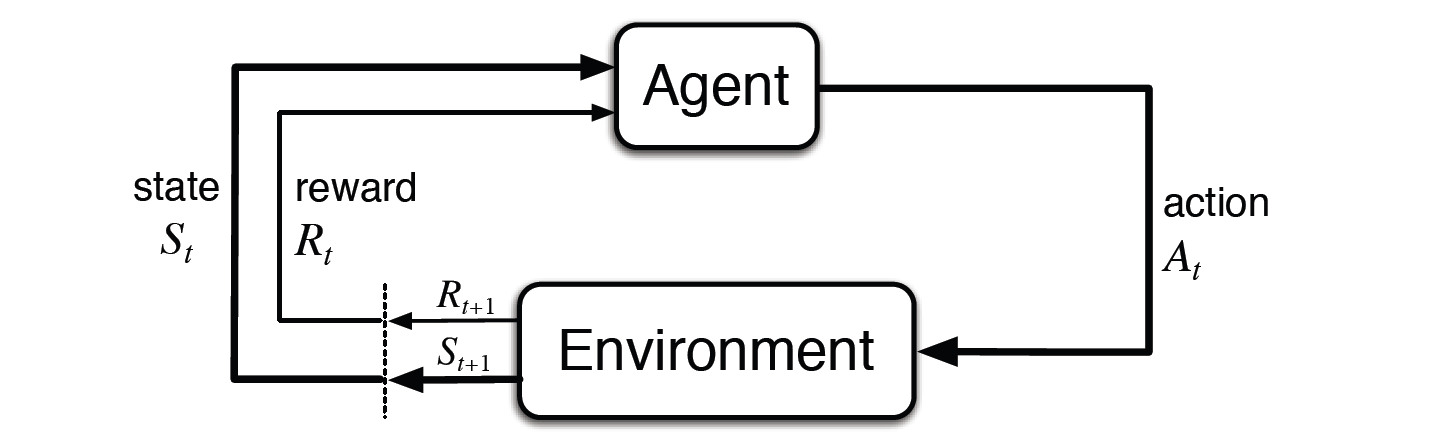
\includegraphics[clip, angle=0, width=12cm]{figures/Loop.png}
\label{fig:1}
\end{figure}
\begin{center}
	{Source: \cite{sutton1998introduction}}
\end{center}

At a sequence of discrete time steps $t = 0,1,2,3...$, the agent interacts with the environment. At each step $t$, the agent receives state information $S _ { t } \in \mathcal{S}$ and performs an action $A _ { t } \in \mathcal { A } ( s )$. As a consequence of the action, the agent receives a reward $R _ { t + 1 } \in \mathcal { R } \subset \mathbb { R }$ and transitions to a new state $S _ { t + 1 }$.

In the context of a \textit{Markov} decision process, the future rewards ($R_{t}$) and states ($S_{t}$) only depend on the previous state and action. 

The general reinforcement learning paradigm involves finding an optimal policy $\pi$ to maximise the expected discounted return. The discount factor is required to ensure that rewards in the distant future are less valuable than current rewards.

$$
G _ { t } \doteq R _ { t + 1 } + \gamma R _ { t  } + \gamma ^ { 2 } R _ { t + 3 } + \cdots = \sum _ { k = 0 } ^ { \infty } \gamma ^ { k } R _ { t + k + 1 }
$$

Value and action-value functions allow the actions of the agent to be assessed under the implementation of a particular policy. The value function and action-value functions respectively are defined below:

$$
\begin{aligned}
v _ { \pi } ( s ) \doteq \mathbb { E } _ { \pi } \left[ G _ { t } | S _ { t } = s \right] = \mathbb { E } _ { \pi } \left[ \sum _ { k = 0 } ^ { \infty } \gamma ^ { k } R _ { t + k + 1 } | S _ { t } = s \right] , \text { for all } s \in \mathcal{S} \\
q _ { \pi } ( s , a ) \doteq \mathbb { E } _ { \pi } \left[ G _ { t } | S _ { t } = s , A _ { t } = a \right] = \mathbb { E } _ { \pi } \left[ \sum _ { k = 0 } ^ { \infty } \gamma ^ { k } R _ { t + k + 1 } | S _ { t } = s , A _ { t } = a \right]
\end{aligned}
$$ 

Ideally, the value function is decomposed into the following (known as the \textit{Bellman's Equation}):

$$
\begin{aligned} v _ { \pi } ( s ) & \doteq \mathbb { E } _ { \pi } \left[ G _ { t } | S _ { t } = s \right] \\ & = \mathbb { E } _ { \pi } \left[ R _ { t + 1 } + \gamma G _ { t + 1 } | S _ { t } = s \right] \\ & = \sum _ { a } \pi ( a | s ) \sum _ { s ^ { \prime } } \sum _ { r } p \left( s ^ { \prime } , r | s , a \right) \left[ r + \gamma \mathbb { E } _ { \pi } \left[ G _ { t + 1 } | S _ { t + 1 } = s ^ { \prime } \right] \right] \\ & = \sum _ { a } \pi ( a | s ) \sum _ { s ^ { \prime } , r } p \left( s ^ { \prime } , r | s , a \right) \left[ r + \gamma v _ { \pi } \left( s ^ { \prime } \right) \right] , \quad \text { for all } s \in S \end{aligned}
$$

Both expressions relate to a specific state and action taken at any time $t$.

A reinforcement learning problem principally involves pursuing the optimal policy $\pi$ which is said to maximise the value and action-value functions:

$$
\begin{aligned}
v _ { * } ( s ) &\doteq \max _ { \pi } v _ { \pi } ( s )\\
q _ { * } ( s , a ) &\doteq \max _ { \pi } q _ { \pi } ( s , a )
\end{aligned}
$$

In the most simple cases where the value and action-value functions are specified, dynamic programming can be used to derive the optimal policy $\pi$.

In the algorithmic trading problem, the value function cannot be ascertained easily in this way. To deal with these situations and arbitrarily large state space, approximate solution methods must be used. This is known as a partially observable Markov decision process as the state is only observed indirectly and cannot be fully known (we cannot know the trading behaviour of other agents for example) and we do not have access to the transition probabilities between states.

Q-Learning is a technique whereby the value functions are repeatedly estimated based on the rewards of our actions and assumes no prior model specification.

\section{Q-Learning} 

Q-learning attempts to estimate $q_{*}$ (optimal action-value function) without any regard for the policy followed. From a high-level perspective, the Q-Learning algorithm proceeds by randomly initialising $Q$, perform actions, measure reward and update $Q$ accordingly (see Figure \ref{fig:ql}). The final output after a training period should be a stable approximation of the $q_{*}$.

\begin{figure}[h!]
	\centering
	\caption{Q-Learning Algorithm}
	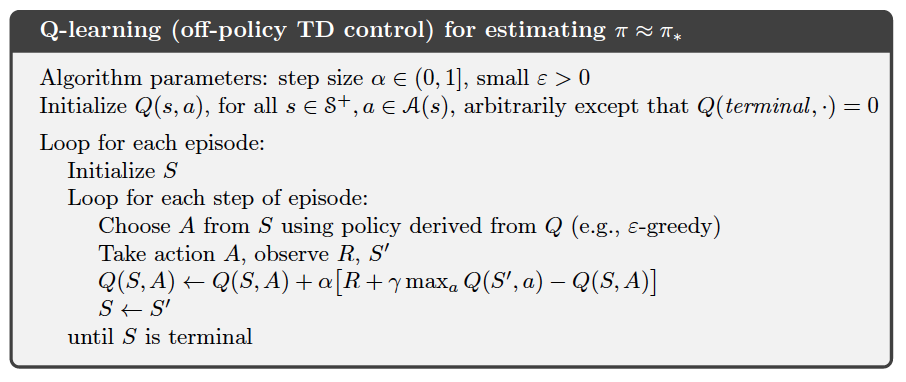
\includegraphics[clip, angle=0, width=13cm]{figures/psudo_code.png}
	\label{fig:ql}
\end{figure}
\begin{center}
	{Source: \cite{sutton1998introduction}}
\end{center}

Notice the Bellman equation appearing in the update phase of the algorithm.

\section{Deep Q Learning}
An extension of this idea (which we aim to employ) is to use neural networks to approximate the Q-function ($Q(s, a)$). In situations where the state space is enumerable, we can produce a Q table which specifies the action-value function for each possible state. However, if the state space is intractable or very large, this is generally not possible or computationally intensive. A neural network is an appropriate tool for our use case due to the infinite nature of the state space. Estimating a table corresponding to every possible state would be excessive in regards to memory requirements.

To train the neural network on the state space, we must define a loss function. The Bellman Equation defines the optimal result; thus we can use this to calculate our loss as follows:

$$
\begin{aligned}
\hat { Q } ( s , a ) &= R ( s , a ) + \gamma \max _ { a ^ { \prime } \in A } Q ( s , a ) \\
\text {Loss} &= \| Q - \hat { Q } \| _ { 2 }
\end{aligned}
$$

In general, a partition of the data is used to train the neural network and approximate the $q_{*}$ function, and this is then used as our action-value function for deciding the optimal policy.

A neural network with two hidden layers is implemented using Tensorflow\footnote{TensorFlow is a free and open-source software library for dataflow and differentiable programming across a range of tasks.} in our case.

\subsection{Problem Formulation - Algorithmic Trading}
Now we must formulate the trading problem as a Markov Decision Process and define the states, actions and rewards \citep{xiong2018practical}.

\begin{itemize}
	\item State: $\mathcal{S} = \{prices,holdings,balance\} $ where $prices$ refers to the current prices of all the stocks in our portfolio, $holdings$ the quantity of each stock held and $balance$ as the total portfolio value. In our simple variant, we are only trading one stock but include a history of prices also (default 200)
	\item Actions: $\mathcal{A} = \{buy,sell,hold\}$ For simplicity and computational tractability, we restrict our action space to buy 1 stock, sell 1 stock or hold.
	\item Rewards: $R_{t} \in \mathcal{R}$ can be defined as the change in the portfolio value due to an action $A_{t}$. Our Reward was defined as $R_{t} = balance_{t} - balance_{t-1}$
	\item Policy: $\pi$ which is governs the trading strategy at state $S$. We converge on the optimal policy by approximating the $q_{*}$ function.
	\item Action-value function: $q_{\pi}(s,a)$ as defined above. The expected reward we obtain by following policy $\pi$, choosing action $A$ while in state $S$. The action-value function is approximated by a neural network.
\end{itemize}



No transaction cost is considered in this study, and the algorithmic trader can only trade with a single stock, Apple (AAPL) or Wawel (WWL). Furthermore, a negative portfolio is not permissible ($balance_{t} \geq 0$ for all $t$) and the trader can only sell owned stock ($holdings_{t} \geq 1$). In our primary model, the initial $balance_{0}$ is set to \$1000 and $price_{0}$ to the price of the stock at our chosen start time $t_{0}$ 

\section{Data, Settings and  Results}

The proposed deep Q-learning system is evaluated on two stocks: Apple (AAPL) and Wawel (WWL). We first describe the data and configurations of the experiment and then present the performance results.

\subsection{Data and Settings}

The databases used in the experiment involve nine years of daily data on Apple and Wawel stocks\footnote{All data was downloaded using Yahoo finance}, ranging from  2010-01-01 through 2019-03-01. The databases are divided into training data sets (2010-01-01 --- 2012-04-13) and test sets (2012-04-16 --- 2019-02-28). Only the daily closing price is used in this study, though other features can be easily incorporated into the model.

We compare the deep Q-learning system with two benchmark strategies: a random decisions policy (RAND) and a buy-and-hold (BH) strategy. For deep Q-learning, the training datasets are used to initialise the deep Q-network, and then the system runs in an online fashion where trading decision making and model adaptation are conducted simultaneously. For the Q-learning part, the discount factor is set to $\gamma =  0.5$. For the deep-learning part, the architecture of the deep Q-network involves four layers in total (two are hidden). The input units (features) are composed by the current budget ($balance_{t}$), the current number of stocks held ($holdings_{t}$) and 200 days of stock history while the output units correspond to the three actions in trading (see Figure \ref{fig_ss_nn}). The learning rate for Q-network is 0.01, and the training stops after 5 epochs. Furthermore, we introduce a new hyper-parameter $\epsilon$ (set at $\epsilon = 0.9$) to keep our solution from getting ``stuck'' when applying the same action over and over. Thus the algorithm exploits the best option with probability $\epsilon$ and explores a random option with probability $1 - \epsilon$.
	
\begin{figure}[h!]
	\begin{center} 
	\caption{The architecture of the deep Q-network and the rolling window scheme}
	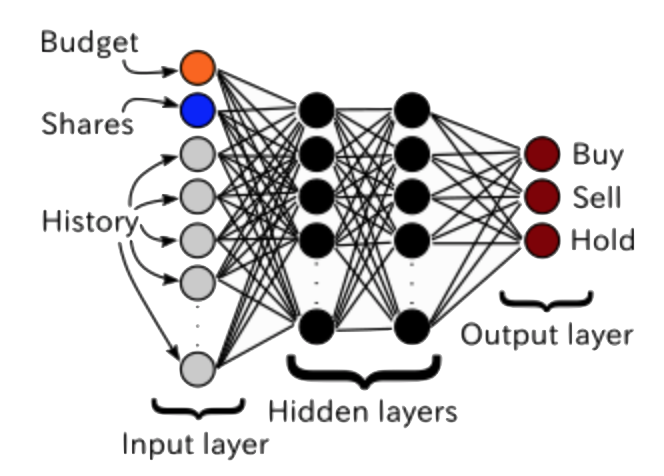
\includegraphics[scale=0.6]{figures/ss_nn.png}
	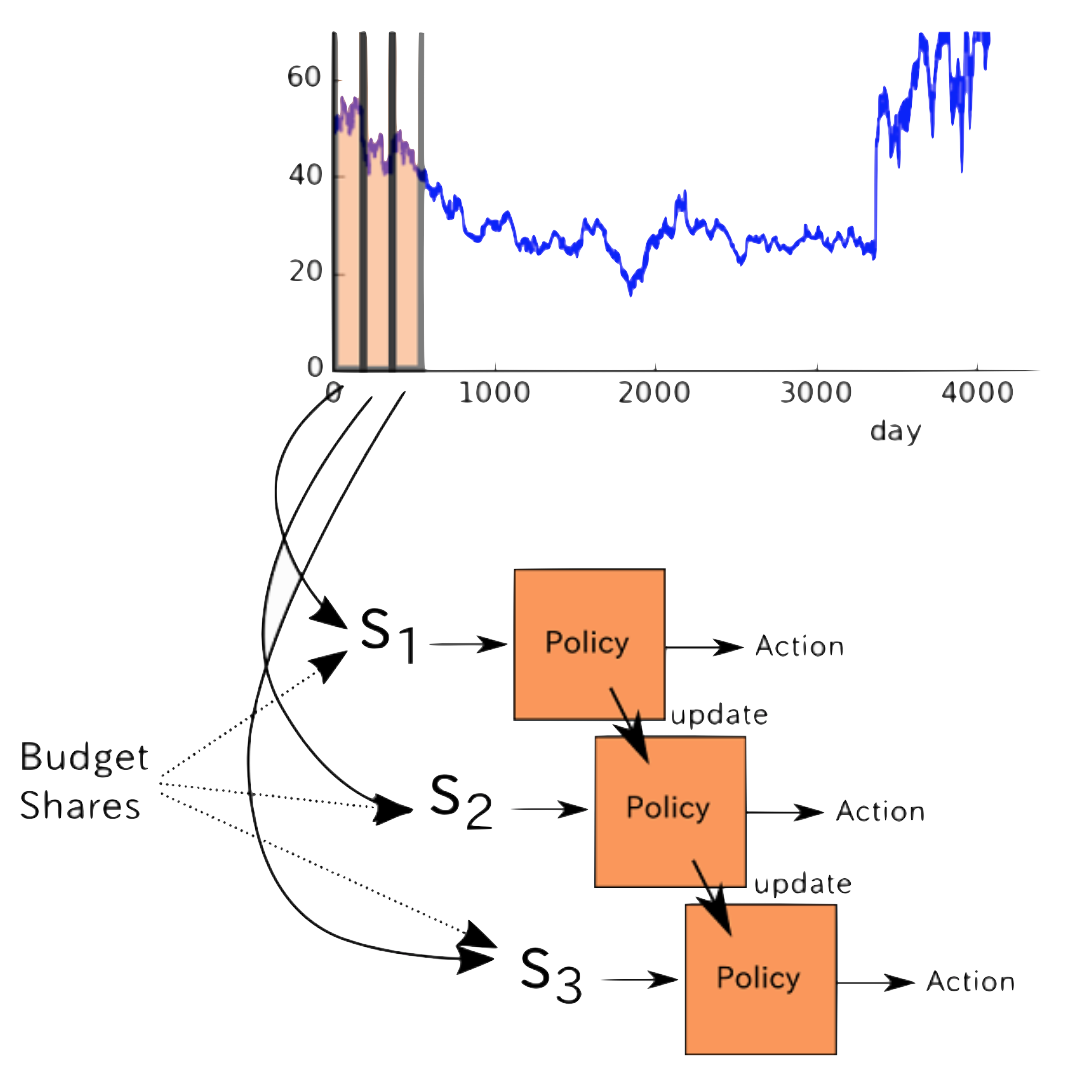
\includegraphics[scale=0.4]{figures/roling_window.png}
	\label{fig_ss_nn}
	\end{center} 
\end{figure}

As mentioned above, to ensure that the Q function is being learned correctly and trending towards an optimal policy, we train the neural network over five epochs. From the plot below (Figure \ref{fig:conver}), the final portfolio value achieved continues to increase, signalling convergence towards an optimal policy. The hyper-parameters were tuned to derive maximum gain. 

\begin{figure}[H]
	\centering
	\caption{Illustrative convergence of the deep Q-network}
	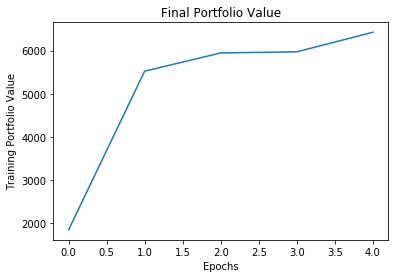
\includegraphics[clip, angle=0, width=10cm]{figures/training.png}
	\label{fig:conver}
\end{figure}

\subsection{Results}

The results of the three trading approaches (BH, RAND, and Deep Q-learning) on the AAPL test set are presented in Figure \ref{fig:aapl}, and the results on the WWL test set are shown in Figure \ref{fig:wwl}. In each figure, the green line illustrates the Deep Q-learning decision policy while the red and blue lines depict the BH and RAND strategies respectively. It can be seen that on both of the two test sets, the deep Q-learning system accumulates more value than the other two systems. A more detailed numerical comparison is shown in Table \ref{table-1} where we report two widely used measures for stock trading: accumulated return and the Sharpe ratio. The Sharpe ratio is defined as:
$$
\text {Sharpe Ratio} = \frac { R _ { p } - R _ { f } } { \sigma _ { p } }
$$
where $R_{f}$ is the risk-free rate (assumed to be 8\%), $R_{p}$ the return of the portfolio and $\sigma_{p}$ is the standard deviation of the portfolio. A larger Sharpe Ratio indicates that the portfolio achieves a better return for its volatility. In a practical setting, this would be an attractive feature for a potential investor. Thus, it can be seen that our deep Q-learning system outperforms the other two methods in terms of total return and the Sharpe Ratio.

\begin{table}[h!]
	\centering
	\caption{Comparison of Trading Performance}
	\label{table-1}
	\begin{tabular}{lcccccc} \\ \hline\hline
		& \multicolumn{3}{c}{AAPL} & \multicolumn{3}{c}{WLL} \\ \hline
		& DQL & BH & RAND & DQL & BH & RAND \\ \hline
		Accumulated Return(\%) & 1.67 & 1.33 & 0.59 & 0.64 & 0.41 & 0.18 \\
		Sharp Ratio & 0.29 & 0.22 & 0.26 & 0.25 & 0.20 & 0.09 \\\hline\hline
	\end{tabular}
\end{table}

Therefore, the results show our deep Q-learning model performs well on both the two stocks (AAPL being a strong stock with a stable upward trend and WWL being a more volatile stock with no apparent trend). This advantage of deep Q-learning can be attributed to two advantages. One of them is the ability to detect the status of the market from the raw and noisy data, and the other is the online nature that adapts itself to new market status quickly. More interesting observations can be found in the portfolio action plots (see Figure \ref{fig:aaplaction} and Figure \ref{fig:wwlaction}). From the positions held by the Q-learning system, it seems that it has learned how to take different actions in different market situations which can largely be attributed to the power of the deep Q-network in discovering the status of the market from the noisy historical price signals.

\begin{figure}[h!]
	\centering
	\caption{The performance of various trading strategies on AAPL}
	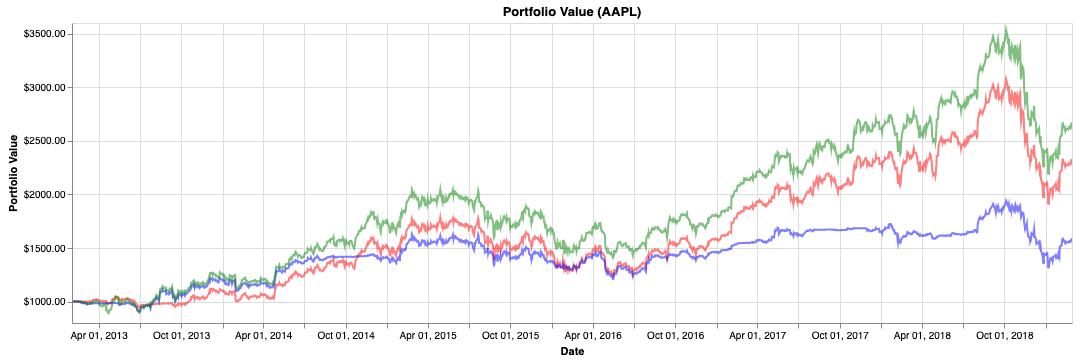
\includegraphics[width=\textwidth]{figures/aapl_portfolio.png}
	\label{fig:aapl}
\end{figure}


\begin{figure}[h!]
	\centering
	\caption{The performance of various trading strategies on WWL}
	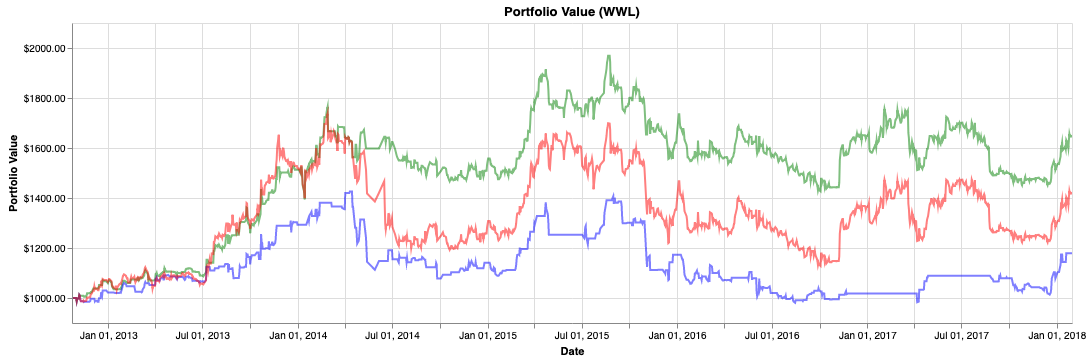
\includegraphics[width=\textwidth]{figures/wwl_portfolio.png}
	\label{fig:wwl}
\end{figure}

\begin{figure}[H]
  \begin{center} 
  	\caption{The positions held by various trading strategies on AAPL}
  	\label{my-label}
	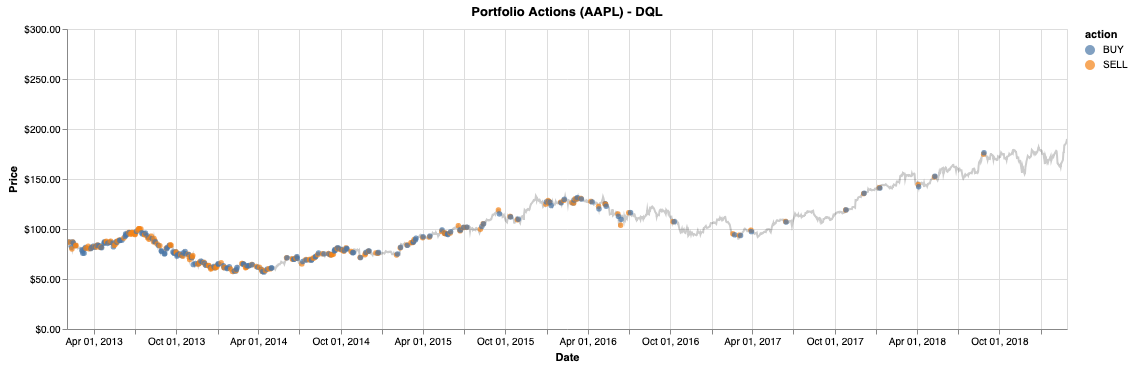
\includegraphics[scale=0.42]{figures/aapl_action_dql.png} \\
	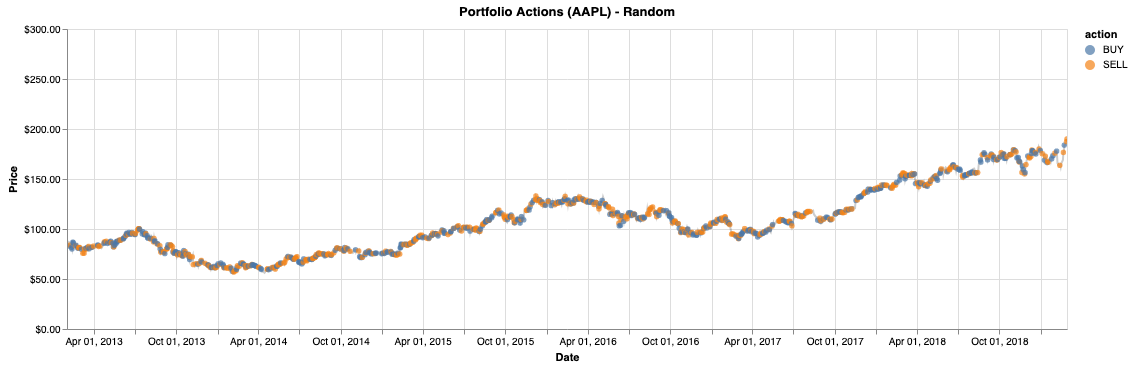
\includegraphics[scale=0.42]{figures/aapl_action_rand.png} \\
	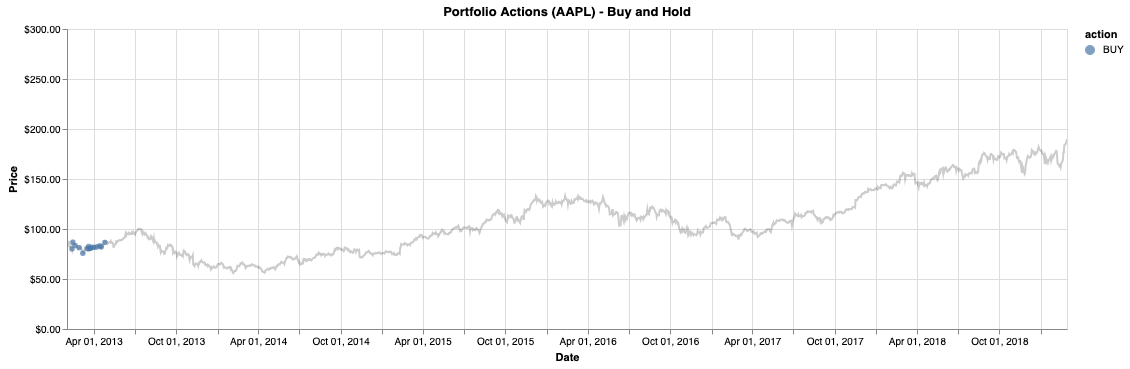
\includegraphics[scale=0.42]{figures/aapl_action_bh.png} \\
	\label{fig:aaplaction}
\end{center} 
\end{figure}

\begin{figure}[H]
  \begin{center} 
  	\caption{The position held by various trading strategies on WWL}
  	\label{my-label}
	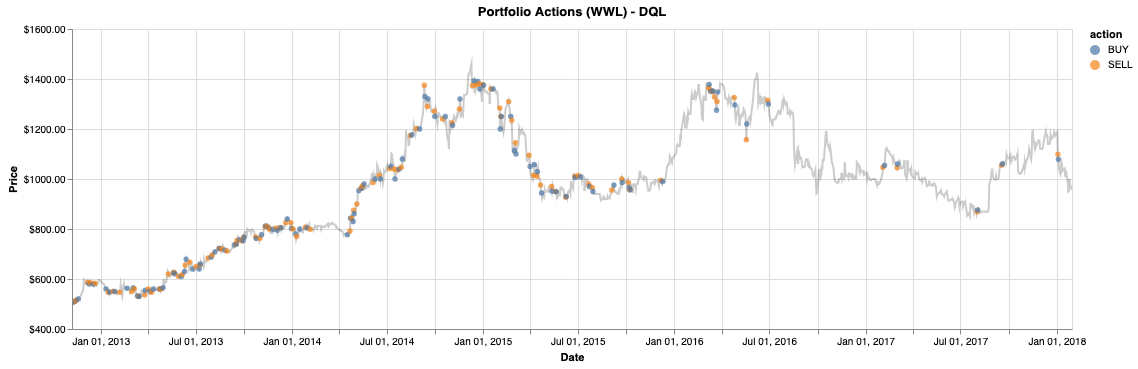
\includegraphics[scale=0.42]{figures/wwl_action_dql.png} \\
	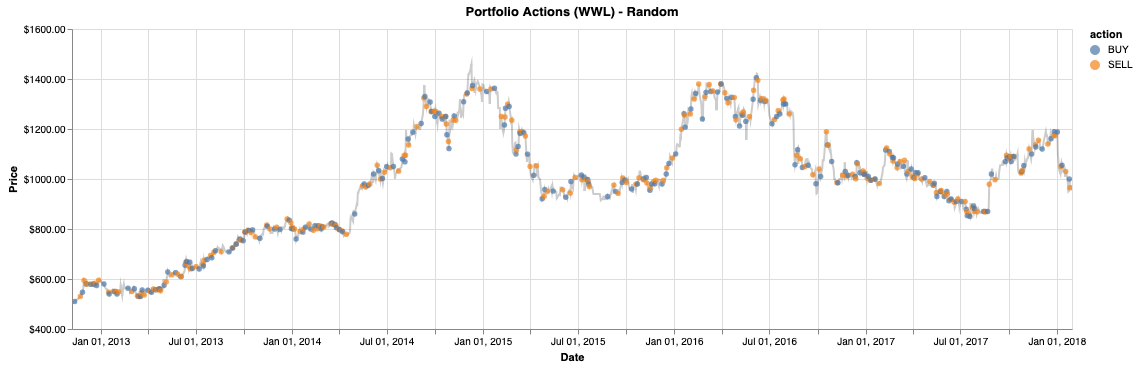
\includegraphics[scale=0.42]{figures/wwl_action_rand.png} \\
	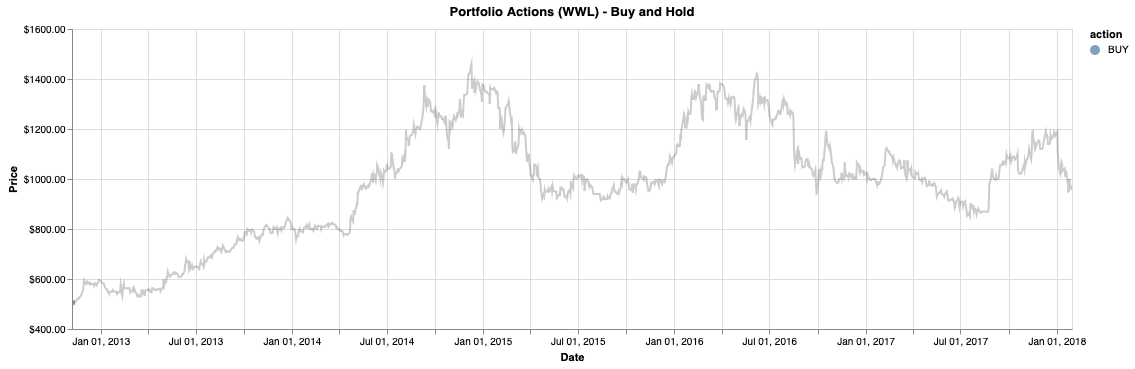
\includegraphics[scale=0.42]{figures/wwl_action_bh.png} \\
	\label{fig:wwlaction}
\end{center} 
\end{figure}

\section{Conclusion}

The investigation aimed to implement reinforcement learning in the context of stock trading. A deep Q-Learning approach was used to approximate the Q-function (action-value function) and develop a trading policy. Through our experiments with AAPL and WLL stocks, we have managed to show that with minimal training and hyper-parameter tuning, our agent can outperform random actions and a Buy and Hold strategy. We have also demonstrated the agent's ability to manage the volatility of the portfolio effectively. There are many possible future developments that could be explored such as using multiple stocks, modifying the reward function and doing further hyper-parameter tuning. Furthermore, the initial budget appeared to be a strong determinant of the behaviour of our agent. A more thorough investigation into this and its implications for algorithmic trading would be an interesting extension.

%_______________________________________________________________________________________________________%
%BIBLIOGRAPHY
%_______________________________________________________________________________________________________%
\pagebreak
\bibliographystyle{agsm}
\setcitestyle{authoryear}
\bibliography{smo.bib}



\end{document}


Despite the algorithm performing well, the \textit{Buy and Hold} strategy also performs similarly as AAPL is a strong stock with a stable upward trend.

To highlight the strength of Q-learning more effectively, we compared the algorithms behaviour on a more volatile stock, where \textit{Buy and Hold} should be less effective.

One of the noticeable strengths of the Q-Learning approach is its control of the volatility (captured by the Sharpe Ratio).
